\chapter{Background} \label{chap:background}

In this section, we will introduce the background leading to the experiment. For example, the different kinds and types of web frameworks. We will also introduce the environment leading to the experiment.

\section{Expanding on the Experiment Background}

From the above section, we stated that during the framework benchmarking experiment, we expect the WebAssembly framework to come out on top from various benefits it provides, such as a lower computation overhead and better RTT delays.

Our experiment will first be conducted in a controlled environment. Depending on the result we receive from this investigation stage, we then decide what the next phase of our experiment will be. This can either be designing, implementing and carrying out a "real-life" scenario experiment with both frameworks. Or to expand, understand and conduct further research into the potential irregularities observed within the collected data from the first stage of the investigation.

This way, we will be extra confident with the data we collected from the experiment. Therefore, we shall have a stronger argument when communicating our results and findings to other researchers and engineers, as well as ensuring that the results we get are as accurate as possible.

\section{Further Understanding of client-side application and server-side application}

A web framework, sometimes also referred to as a web application framework, is a collection of functionalities and libraries engineered and designed to lay the groundwork and provide basic infrastructures and logic for applications to be built on top of. This way, developers and engineers working on the project do not have to implement such functionalities themselves. It simplifies the development process, reduces development time and increases development productivity output \cite{exp11}.

There are usually two web framework categories: \textbf{client-side} and \textbf{server-side}. The former is generally used in order to construct dynamic web applications \cite{exp12}, while the latter is usually used to develop backend API services. According to the \textbf{2022 annual developer survey from stack overflow} \cite{exp20}, some of the most popular client-side frameworks including \textbf{React.js} \cite{exp13}, \textbf{Angular} \cite{exp14} and \textbf{Vue.js} \cite{exp15}, while some of the most popular server-side frameworks including \textbf{Node.js} \cite{exp16}, \textbf{ASP.NET} \cite{exp17} and \textbf{Django} \cite{exp18} (server-side Django REST framework) \cite{exp19}.

It has been mentioned in multiple research articles that running complete web applications using the current cloud solution may produce too much overhead, thus leading to inefficiency. For example, Gackstatter \cite{exp21} recognises the limitation of today's "cloud-centric model" when it comes to deploying web applications at the edge. Specifically, the author stated that applying the current solution, such as virtual machines and containers, does not promise an effective solution due to the limited resources available. Additionally, Gadepalli et al. not only pointed out the wide adoption of the virtual machine/container model, but also stated that server applications built using WASM functions that run naively have the potential to expand the current use case of comprehensive applications running from the edge due to the reduction of the overhead which reduces the response time down to within \textbf{10} milliseconds \cite{exp6}.

With the current model of implementation, \textbf{Docker} \cite{exp22} and \textbf{Kubernetes} \cite{exp23} are usually used in the publishing process to prepare an application for edge deployment. In this case, it would "wrap" the application into containers which will be further deployed onto self-managed serverless infrastructures or cloud computing service providers that provide edge services such as \textbf{Amazon Web Service} or \textbf{Microsoft Azure}. Those services will then distribute the application to edge devices across data centres worldwide.

My research aims to study and uncover the current state of WebAssembly frameworks running on the edge, which is to run functions as microservices directly from the native operating system using WebAssembly through a WASM runtime, and its performance gap and inconsistency with traditional VM-based implementations. This includes applications developed and deployed with virtual machines, containers and conventional language runtimes.

Currently, at this stage, the true performance capability of WebAssembly has yet to be fully realised due to the relatively short time it has been around compared to JavaScript - which has almost \textbf{30} years of development ahead of it. However, it is apparent to us that WebAssembly has a huge potential in terms of its performance both when running in web browsers as well as running on operating systems naively through a runtime. We can back this up with the performance data of JavaScript over the years. In a presentation, Verschore presented a figure which stated that between 2001 and 2009, there was a \textbf{100} times improvement in JavaScript's performance as well as considerable increases in the browser Octane score (web page loading speed) \cite{exp24}.

\bigskip
\begin{figure}[!ht]
\centering
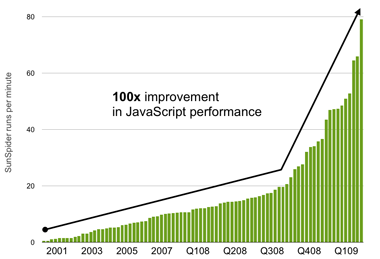
\includegraphics[scale=0.7]{js-perf}
\caption{\footnotesize{SunSpider benchmark score for the SpiderMonkey engine, which is used in Firefox \cite{exp24}}}
\captionsetup{aboveskip=0pt,font=it}
\end{figure}
\bigskip

On top of that, the V8 JavaScript engine \cite{int31} behind popular browsers such as Google Chrome \cite{exp25} and Brave \cite{exp26} also had an incredible journey from when it was first released to the public back in 2008. The V8 development team undertook and released a set of benchmark scores comparing the performance of the Chrome browser from its original beta to the versions in 2018. The results showed that in just 10 years, both its V8 Bench score \cite{exp27} and Speedometer score \cite{exp28} increased by \textbf{4} times, and the engine had also became a lot more stable as well as added support for a lot more chip architectures such as \textbf{ARM} and \textbf{ARM 64} \cite{exp29} \cite{exp30}.

\newpage
\bigskip
\begin{figure}[hp]
\centering
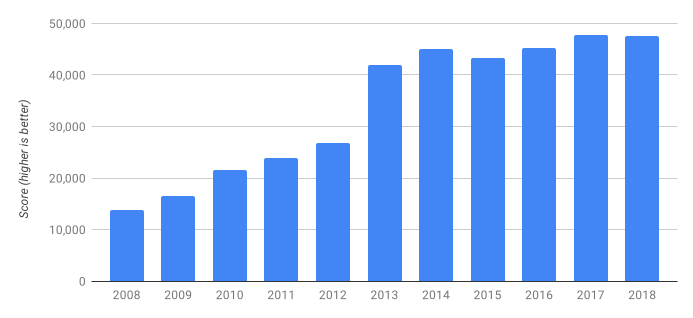
\includegraphics[scale=0.5]{chrome-v8-bench}
\caption{\footnotesize{Google Chrome's V8 Bench score between its original beta and the version in 2018 \cite{exp29}}}
\captionsetup{aboveskip=0pt,font=it}
\end{figure}
\bigskip

\bigskip
\begin{figure}[hp]
\centering
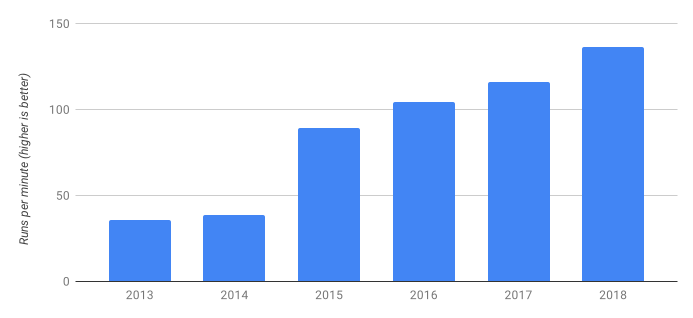
\includegraphics[scale=0.5]{chrome-speedometer-1}
\caption{\footnotesize{Google Chrome's Speedometer 1 score between its original beta and the version in 2018 \cite{exp29}}}
\captionsetup{aboveskip=0pt,font=it}
\end{figure}
\bigskip

One recent example is the new \textbf{Bun.js} JavaScript runtime \cite{exp31}. It is a newly released JS runtime at the time of writing. It was built with prior experience with Node.JS and made several visible improvements on top of that. Namely adding the support for edge computing.

\bigskip
\begin{figure}[hp]
\centering
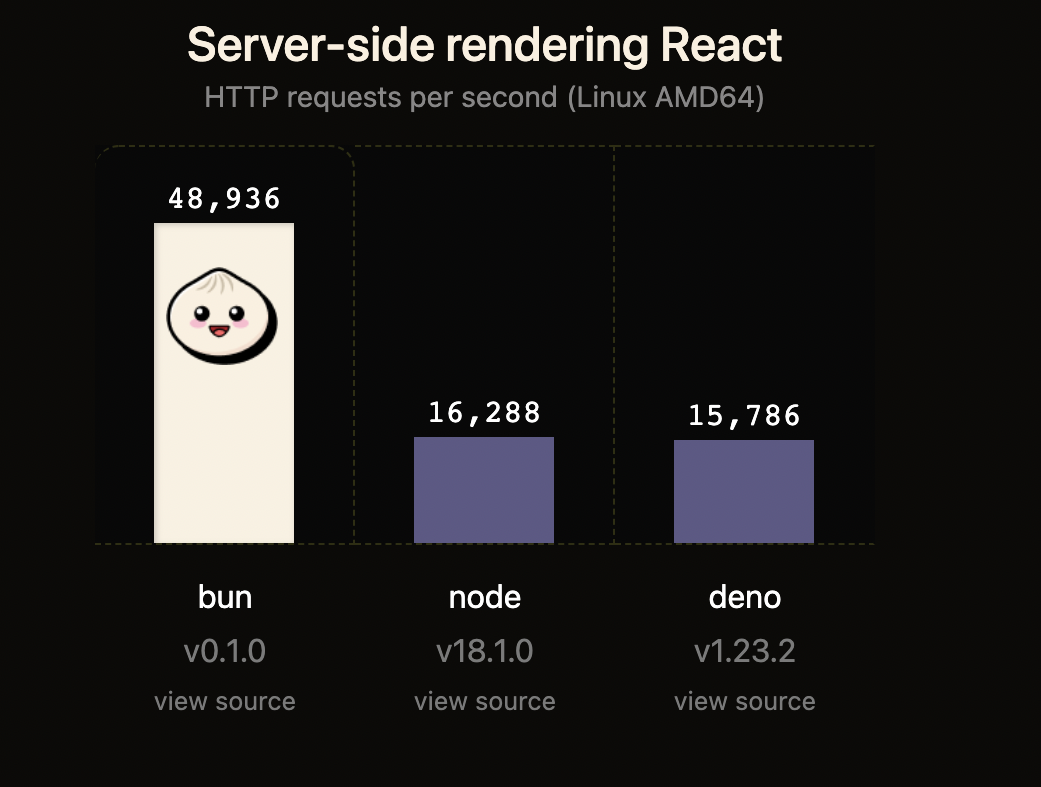
\includegraphics[scale=0.35]{bun-comparison}
\caption{\footnotesize{Performance comparison on HTTP requests between Bun and Node.JS \cite{exp31}}}
\captionsetup{aboveskip=0pt,font=it}
\end{figure}
\bigskip